\documentclass[
    10pt,
    pdf,
    UTF8,
    aspectratio=169
]{ctexbeamer}

% font settings
% https://latex-beamer.com/
% \usetheme{Copenhagen}
% \useinnertheme{default}
% \setCJKsansfont{\CJKfamily{zhkai}}
% \usefonttheme{\kaishu}
%% English fonts
\usefonttheme{serif}
% \usepackage{times}
%% math fonts
\usefonttheme{professionalfonts}
%% Chinese fonts
\setbeamerfont{title}{family=\heiti}
\setbeamerfont{author}{family=\kaishu, size=\large}
\setbeamerfont{institute}{family=\kaishu}
\setbeamerfont{date}{family=\songti, size=\scriptsize}
\setbeamerfont{section in toc}{family=\heiti, size=\large}
\setbeamerfont{subsection in toc}{family=\heiti}
\setbeamerfont{frametitle}{family=\heiti}
\setbeamerfont{footnote}{family=\fangsong,size=\scriptsize}
\setbeamerfont{caption}{family=\fangsong}
% TODO
% \setbeamerfont{subcaption}{family=\fangsong}
\setbeamerfont{abstract title}{family=\songti}
\setbeamerfont{abstract}{family=\kaishu}
\setbeamerfont{block title}{family=\songti}
\setbeamerfont{block body title}{family=\songti}
\setbeamerfont{block body example}{family=\kaishu}
% TODO, can't work
% \setbeamerfont{block body definition}{family=\kaishu}
% \setbeamerfont{definition body}{family=\kaishu}

% shape
% shape
% more details, see % https://zhuanlan.zhihu.com/p/138021900
\setbeamertemplate{section in toc}[square]
\setbeamertemplate{subsection in toc}[square]

\setbeamertemplate{enumerate subitem}{\arabic{enumi}}
\setbeamertemplate{enumerate subitem}{\alph{enumii}}
\setbeamertemplate{enumerate subsubitem}{\roman{enumiii}}
\setbeamertemplate{itemize item}[square]
\setbeamertemplate{itemize subitem}[triangle]
\setbeamertemplate{itemize subsubitem}[circle]
\setbeamertemplate{blocks}[rounded][shadow=true]
% TODO
% \setbeamertemplate{title page}[rounded][shadow=true]
\setbeamertemplate{footline}[frame number]
\setbeamertemplate{caption}[numbered]
% TODO can't work
% \setbeamertemplate{caption}{\insertcaptionnumber sd \insertcaptionname}

% color
% color
% https://zhuanlan.zhihu.com/p/137877025
\definecolor{ScutColor1}{RGB}{0, 70, 144}
\definecolor{ScutColor2}{RGB}{0, 110, 180}
\definecolor{ScutColor3}{RGB}{100, 150, 200}
\setbeamercolor{structure}{fg=ScutColor1} % witout bg=white

\setbeamercolor{title}{fg=white,bg=ScutColor1}
\setbeamercolor{section in toc}{fg=ScutColor1, bg=white}
\setbeamercolor{subsection in toc}{fg=ScutColor2, bg=white}
\setbeamercolor{block title}{fg=white, bg=ScutColor2}
\setbeamercolor{block body}{fg=black,bg=gray!10}
\setbeamercolor{block title alerted}{fg=white,bg=red!75!black}
\setbeamercolor{block body alerted}{fg=black,bg=red!5}
\setbeamercolor{block title example}{fg=white,bg=green!50!black}

% package
% figure
\usepackage{graphicx}
\usepackage[]{subfig}
\usepackage{tikz}

% layout
\usepackage{multicol}
\usepackage{multirow}

% code
\usepackage{minted}
% Algorithm
%% Float of algorithm
\usepackage{algorithm}
%% Body of algorithm
\usepackage{algorithmic}
%% Custom setting for algorithmic
\renewcommand{\algorithmicrequire}{\textbf{Input:}} 
\renewcommand{\algorithmicensure}{\textbf{Output:}}

% reference
\usepackage[style=ieee]{biblatex}
\addbibresource{ref.bib}
\usepackage{hyperref}

% math
%% package for math
\usepackage{amssymb,amsmath}
\newcommand{\vect}[1]{\boldsymbol{#1}} % vector
\newcommand{\mat}[1]{\mathbf{#1}}      % matrix
\newcommand{\tensor}[1]{\mathsf{#1}}   % tensor
\newcommand{\set}[1]{\mathbb{#1}}      % set
\newcommand{\T}{\mathrm{T}}            % transposition
\everymath{\displaystyle}              % block style

\title{中文 Latex PPT 模板}
\subtitle{一个用于学术展示的 PPT}
\author{姓名}
\institute{华南理工大学}
\date{\today}
\logo{
    % https://latex-beamer.com/tutorials/logo-beamer/
    \begin{tikzpicture}[overlay,remember picture]
        \node[left=0.015\textwidth] at (current page.26){
          
\includegraphics[width=0.05\textwidth]{img/logo-short.png}
        };
    \end{tikzpicture}
}
\titlegraphic{
    
\includegraphics[width=0.4\textwidth]{img/logo.png}
}

\begin{document}

\kaishu
\begin{frame}
    \titlepage
\end{frame}

\begin{frame}
    \frametitle{目录}
    \tableofcontents[subsectionstyle=hide]
\end{frame}

\AtBeginSubsection[]
{
    \begin{frame}
        \frametitle{目录}
        \transfade
        \tableofcontents[sectionstyle=show/shaded,subsectionstyle=show/shaded/hide]
    \end{frame}
}

\section{\LaTeX 相关}

\subsection{列表}

\begin{frame}
    \frametitle{无序列表}
    \begin{itemize}
        \item 无序列表 1
        \begin{itemize}
            \item 无序列表 1.1
            \item 无序列表 1.2
            \item 无序列表 1.3
            \begin{itemize}
                \item 无序列表 1.3.1
                \item 无序列表 1.3.2
                \item 无序列表 1.3.3
            \end{itemize}
        \end{itemize}
        \item 无序列表 2
        \item 无序列表 3
    \end{itemize}
\end{frame}
\begin{frame}
    \frametitle{有序列表}
    \begin{enumerate}
        \item 有序列表 1
        \begin{enumerate}
            \item 有序列表 1.1
            \item 有序列表 1.2
            \item 有序列表 1.3
            \begin{enumerate}
                \item 有序列表 1.3.1
                \item 有序列表 1.3.2
                \item 有序列表 1.3.3
            \end{enumerate}
        \end{enumerate}
        \item 有序列表 2
        \item 有序列表 3
    \end{enumerate}
\end{frame}
\begin{frame}
    \frametitle{说明性列表}
    \begin{description}
        \item[名词 1] 名词 1 的解释
        \item[名词 2] 名词 2 的解释
    \end{description}
\end{frame}

\subsection{文字}

\begin{frame}
    \frametitle{字体}
    \begin{columns}
        \begin{column}{0.2\textwidth}
            \begin{itemize}
                \item {\songti 宋体}
                \item {\heiti 黑体}
                \item {\fangsong 仿宋}
                \item {\kaishu 楷书}
                % \item {\lishu 隶书}
                % \item {\youyuan 幼圆}
                % \item {\yahei 雅黑}
                % \item {\pingfang 苹方}
            \end{itemize}
        \end{column}
        \begin{column}{0.4\textwidth}
            \begin{itemize}
                \item {\tiny tiny}
                \item {\scriptsize scriptsize}
                \item {\footnotesize footnotesize}
                \item {\normalsize normalsize}
                \item {\large large}
                \item {\Large Large}
                \item {\LARGE LARGE}
                \item {\huge huge}
                \item {\Huge Huge}
            \end{itemize}
        \end{column}
        \begin{column}{0.4\textwidth}
            \begin{itemize}
                % \songti
                \item normal 正常
                \item \textit{italic}: \textit{斜体}
                \item \textsl{slanted}: \textsl{中文}
                \item \textbf{bold}:\textbf{加粗}
            \end{itemize}
        \end{column}
    \end{columns}
\end{frame}

\subsection{图表}

\begin{frame}
    \frametitle{图}
    \begin{figure}
        \centering
        
\includegraphics[width=0.7\textwidth]{./img/logo.png}
        \caption{ 华南理工大学 logo}
        \label{fig:logo}
    \end{figure}
\end{frame}

\begin{frame}
    \frametitle{子图}
    \begin{figure}
        \centering
        \subfloat[\fangsong 子图 1\label{fig:subfig-1}]{
            
\includegraphics[width=0.12\textwidth]{./img/logo-short.png}
        }
        \hspace{1em}
        \subfloat[\fangsong 子图 2\label{fig:subfig-2}]{
            
\includegraphics[width=0.5\textwidth]{./img/logo.png}
        }
        ~\\
        \subfloat[\fangsong 子图 3\label{fig:subfig-3}]{
            
\includegraphics[width=0.5\textwidth]{./img/logo.png}
        }
        \hspace{1em}
        \subfloat[\fangsong 子图 4\label{fig:subfig-4}]{
            
\includegraphics[width=0.12\textwidth]{./img/logo-short.png}
        }
        \caption{子图的 caption 需要自己手动设置为「仿宋」字体}
        \label{fig:subfig}
    \end{figure}
\end{frame}

\begin{frame}
    \frametitle{表}
    \begin{columns}
        \begin{column}{0.3\textwidth}
            \begin{table}
                \centering
                \caption{参数值}
                \label{tb:paramter}
                \begin{tabular}{c|c}
    \hline
    Parameter & Value \\ \hline
    $\alpha$  & 1     \\ \hline
    $\beta$   & 1     \\ \hline
\end{tabular}
            \end{table}
        \end{column}
        \begin{column}{0.7\textwidth}
            \begin{table}
                \centering
                \caption{参数值}
                \label{tb:figure}
                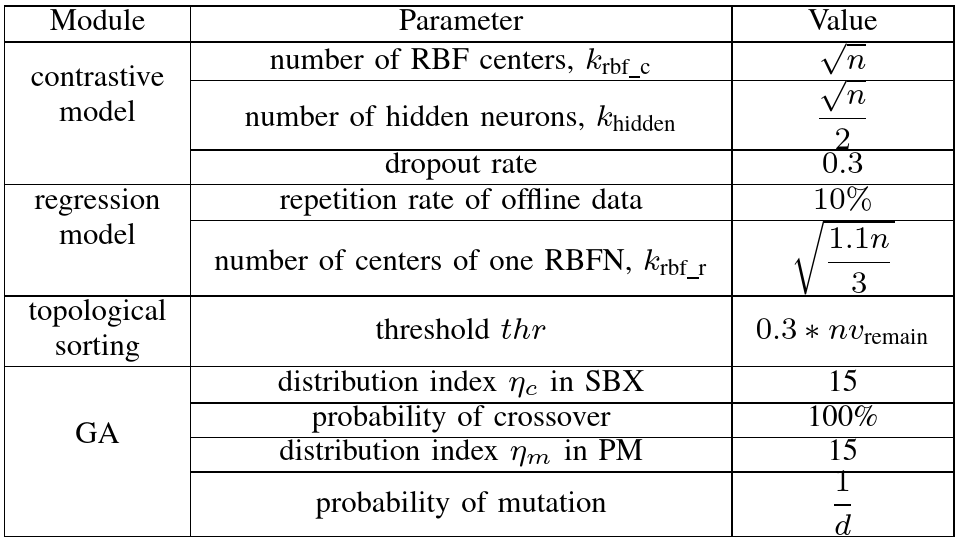
\includegraphics[width=1\textwidth]{./table/figure.png}
            \end{table}
        \end{column}
    \end{columns}
    \hspace{2em} 有时候太懒了,直接截图,把图片扔到 table 环境,例如右边的表。
\end{frame}

\subsection{公式}
\begin{frame}
    \frametitle{公式}
    \begin{block}{行间公式}
        \begin{equation}
            \label{eq:example}
            a_n = a_{n-1} + 1
        \end{equation}
    \end{block}
    \begin{block}{行内公式}
        这是一个简单的等差数列公式 $a_n = a_{n-1} + 1$ 。
    \end{block}
\end{frame}

\section{Beamer 相关}

\subsection{环境}

\begin{frame}
    \frametitle{block}
    \begin{block}{标题}
        \hspace{2em} Block 的内容。
        如果内容比较长的话,可以使用  hpsace\{2em\} 在行首进行缩进两个字符。
    \end{block}
\end{frame}
\begin{frame}
    \frametitle{摘要}
    \begin{abstract}
        摘要的内容
    \end{abstract}
\end{frame}
\begin{frame}[allowframebreaks]
    \frametitle{数学}
    \begin{theorem}[标题]
        主体内容
    \end{theorem}
    \begin{lemma}[标题]
        主体内容
    \end{lemma}
    \begin{proof}[证明(标题)]
        主体内容
    \end{proof}
    \begin{corollary}[标题]
        主体内容
    \end{corollary}
    \begin{example}[标题]
        主体内容
    \end{example}
    \begin{definition}[标题]
        \kaishu 目前定义这里需要手动设置字体为「楷体」。
    \end{definition}
\end{frame}

\begin{frame}
    \frametitle{alertblock}
    \begin{alertblock}{标题}
        主体内容
    \end{alertblock}
\end{frame}

\subsection{分栏}

\begin{frame}
    \frametitle{分栏}
    \begin{columns}
        \column{0.7\textwidth}
        左边占用了 0.7 宽度。
        \column{0.3\textwidth}
        右边占用了 0.3 宽度。
    \end{columns}
\end{frame}

\subsection{脚注}

\begin{frame}
    \frametitle{单栏脚注}
    \hspace{2em} 这是一个简单的 \LaTeX Beamer 中文模板,如果对你有帮助的话。
    麻烦给我 Github \footnote{
        \url{https://github.com/h-hg}
    }加个 Star。

    \hspace{2em} 当然脚注也可以是引用论文 \footfullcite{he2016deep} 的。
\end{frame}

\begin{frame}
    \frametitle{多栏脚注}
    \begin{columns}
        \begin{column}{0.5\textwidth}
            \hspace{2em} 多栏的情况下,脚注默认不会显示在页面的最下面的,例如 \footnote{多栏的默认脚注的位置}。

            \hspace{2em} 脚注论文的引用 \footfullcite{he2016deep} 也是类似的。
        \end{column}
        \begin{column}{0.5\textwidth}
            \hspace{2em} 但是可以通过 [frame] 来解决这个问题,例如 \footnote[frame]{带有 [frame] 的 footntoe}。

            \hspace{2em} 而论文的引用 \footnote[frame]{\fullcite{he2016deep}} 可以配合 fullcite 来实现。
        \end{column}
    \end{columns}
\end{frame}

\section{其他}

\subsection{高亮}

\begin{frame}
    \frametitle{短代码}
    \inputminted[linenos]{cpp}{./code/demo.cpp}
    \hspace{2em} 如果代码比较长,可以选择下面两种方法之一。
\end{frame}

\begin{frame}
    \frametitle{两栏}
    这种通过 multicols 宏包以及改变代码字体大小来实现放在同一页 PPT。
    \begin{multicols}{2}
        \inputminted[linenos,fontsize=\scriptsize]{cpp}{./code/quicksort.cpp}
    \end{multicols}
\end{frame}

\begin{frame}[allowframebreaks]
    \frametitle{多页}
    这种通过允许代码跨多个 PPT 页来实现。
    \inputminted[linenos]{cpp}{./code/quicksort.cpp}
\end{frame}

\subsection{伪代码}

\begin{frame}[allowframebreaks]
    \frametitle{伪代码}
    \begin{algorithm}[H]
        \scriptsize
        \caption{KahnAlgorithm}
        \label{algo:kaha}
        \begin{algorithmic}[1]
    \REQUIRE Graph $G(\mathbb{V}, \mathbb{E})$
    \ENSURE Sequence $L$
    \STATE $L \leftarrow$ an empty sequence
    \STATE $Q \leftarrow$ the vertices whose indegree is zero
    \WHILE{$Q$ is not empty}
        \STATE $u \leftarrow$ remove the top node of $Q$
        \STATE add $u$ to $L$
        \FOR{each node $v$ with an edge $e$ from $u$ to $v$}
            \STATE remove edge $e$ from graph $G$
            \IF{indegree of $v$ is $0$}
                \STATE push $v$ to $Q$
            \ENDIF
        \ENDFOR
    \ENDWHILE
    \RETURN $L$
\end{algorithmic}
    \end{algorithm}
    \begin{columns}
        \begin{column}{0.65\textwidth}
            \begin{algorithm}[H]
                \scriptsize
                \caption{Framework}
                \label{aglo:figure}
                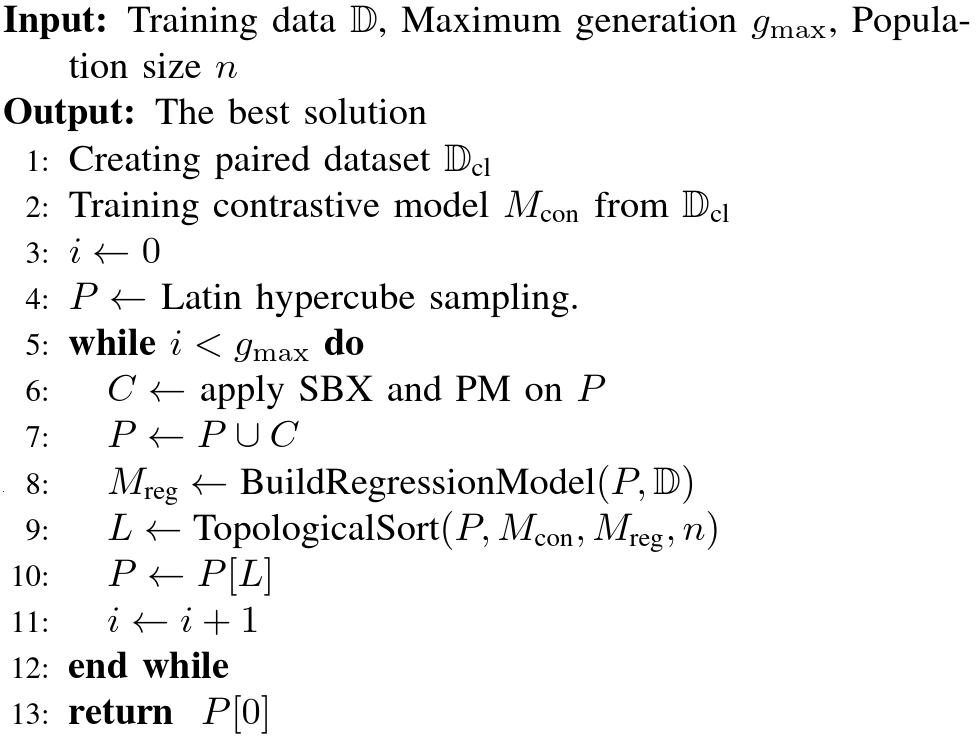
\includegraphics[width=\textwidth]{./algo/figure.png}
            \end{algorithm}
        \end{column}
    \end{columns}
    \hspace{2em} 有时候太懒了,直接截图,把图片扔到 algorithm 环境,例如上面的算法。
\end{frame}


\section*{参考文献}
\begin{frame}[allowframebreaks]
    \frametitle{参考文献}
    \printbibliography
\end{frame}
  
\section*{结束}
\begin{frame}{}
    \centering
    \huge
    谢谢你的聆听!
\end{frame}

\end{document}